\documentclass[a4paper, 12pt]{article}
\usepackage[slovene]{babel}
\usepackage[utf8]{inputenc}
\usepackage[T1]{fontenc}
\setlength{\parindent}{0px}
\setlength{\parskip}{10px}
%standard

\usepackage{listings}
\usepackage{color}
\usepackage{amssymb}
\usepackage{tikz}
\usepackage{pgfplots}
\usetikzlibrary{patterns}
\pgfplotsset{width=7cm, compat=1.10}
\usepgfplotslibrary{fillbetween}

\title{Avditorne vaje za Programiranje II}
\author{Matej Blagšič}

\begin{document}
%--------------------------------------------
\definecolor{dkgreen}{rgb}{0,0.6,0}
\definecolor{gray}{rgb}{0.5,0.5,0.5}
\definecolor{mauve}{rgb}{0.58,0,0.82}
\definecolor{lgray}{RGB}{250,250,250}
%--------------------------------------------
	\lstset{
		frame=l,%single
		language=C,
		aboveskip=3mm,
		belowskip=3mm,
		showstringspaces=false,
		columns=flexible,
		basicstyle={\small\ttfamily},
		numbers=none,
		numberstyle=\tiny\color{gray},
		keywordstyle=\color{blue},
		commentstyle=\color{dkgreen},
		stringstyle=\color{mauve},
		breaklines=true,
		breakatwhitespace=true,
		tabsize=4,
		backgroundcolor=\color{lgray},
		moredelim=**[is][\color{dkgreen}]{@}{@}
	}
%-------------------------------------------

%-------------------------------------------
	\maketitle
	\thispagestyle{empty}
	\pagebreak
	\setcounter{page}{1}
%-----------------------------------Tu naprej

\begin{center}
\textbf{Pomembno}
\end{center}
Te vaje so direktno iz pouka. Koda morda ni identična od te asistena, ampak deluje enako. Prav tako je komentirana in obrazložena skupaj z navodili in opazkami za lažje razumevanje kode. Prav tako se sklicujem in že tu pozivam, da si pogledaš zapiske iz pouka, ki so kot nekakšen učbenik. Notri je snov, teorija in primeri iz pouka. Prijetno branje in učenje želim!

\section*{1. vaja}
/empty/
\section*{2. vaja}

\underline{Izračunaj $\int_{x_0}^{x_1}\, 2x^2-5x\, dx$. Rezultat preveri analitično.}	\

Če analitično integriramo itegral, dobimo: $\int_{x_0}^{x_1}\, 2x^2-5x\, dx = 2\frac{x_1^3}3-5\frac{x_0^2}2$\

Sedaj spišimo kodo:
\begin{lstlisting}
int main(){
	float x, x0, x1;
	float dx = 0.0000001;
	float integral = 0;
	printf("vnesi spodno mejo");
	scanf("%f",&x0);
	printf("Vnesi zgornjo mejo");
	scanf("%f",&x1);

	for(x=x0; x<x1;x+=dx){
		integral += dx*(2*x*x-5*x);
	}

	printf("Integral znasa: %f\n", integral);
	return 0;
}
\end{lstlisting}
Pri programu nam spremenljivka dx sporoči, kako širok del območja integrira. Manjša, kot je cifra, bolj natančno izračuna. x0 in x1 sta spodnja in zgornja meja integracije, x pa je spremenjivka, ki jo premikamo po intervalu za dx razdaljo in seštevamo pravokotnike.
	
\begin{figure}[!htbp]
	\centering
	\caption{Integracije funkcije na intervalu $[a, b]$}
	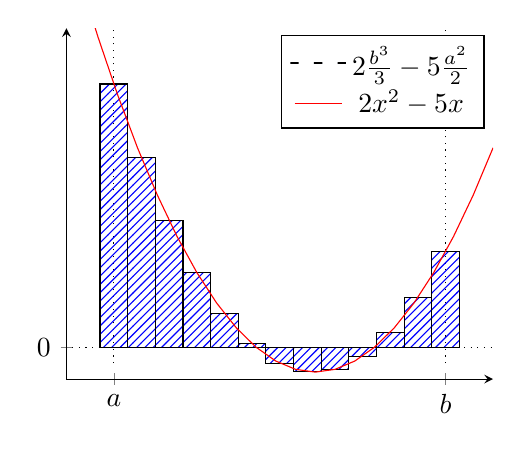
\begin{tikzpicture}
	\begin{axis}[axis lines=left,xmin=-4,xmax=5,ymin=-4,ymax=40,ytick={0}, yticklabel={$0$},xtick={-3,4},xticklabels={$a$,$b$}]
		\addplot[dotted]{0};
		\addplot+[mark=none, dotted, color=black] coordinates {(-3, -2)(-3,40)};
		\addplot+[mark=none, dotted, color=black] coordinates {(4, -2)(4,40)};
		\addplot[domain=-3:4, ybar, samples=13, pattern = north east lines, pattern color=blue]{2*x*x-5*x};
		\addplot[color = red]{2*x*x-5*x};
		\legend{,,,$ 2\frac{b^3}3-5\frac{a^2}2$, $2x^2-5x$}
	\end{axis}
	\end{tikzpicture}
\end{figure}
	
\section*{3. vaja}
\subsection*{1. naloga}

\underline{Napiši program, ki izpiše in izračuna faktorielo(fakulteta) nekega števila(1-20)}\

Pri temu programu spoznamo omejitve velikosti spremenljivk. Pomemno je, da so števila, ki jih hočemo hraniti in predstavljani v polni natančnosti ne presegajo velikosti spremenljivke. Če ne, potem se prične pačenje podatkov. Vidimo, da lahko uporabimo izrad long long in s tem povečamo obseh navadnega long tipa. Podobno lahko naredimo tudi s spremenljivkam s plavajočo vejico, recimo \lstinline|long double|.

\pagebreak

\begin{lstlisting}
int main(){
	unsigned long long resitev = 1, n;

	for(n=1; n<=20; n++){
		for(int i=1; i<=n; i++){
			resitev *= i;
		}
		printf("Faktoriela od %lld! je %lld\n", n, resitev);
		resitev = 1;
	}
	return 0;
}
\end{lstlisting}

\subsection*{2. naloga}
	
\underline{Napiši program, ki sešteje maso lune in zemlje ter sonca.}\

Namen vaje je dodatno spoznati omejitve spremenljivk v programskem jeziku C. Mase lune, zemlje in sonca so ogromne, zato se začenja poznati popačenje podatkov. Ugotovili smo, da dobimo kar se da dobre rezultate, če uporabimo \lstinline|double|, ki ima največji obseh, a se vseeno na določenem mestu pojavi naključna številka, ki ni podana med vhodnimi podatki.

\begin{lstlisting}
int main(){
	double luna = 7.348e22;
	double zemlja = 5.972e24;
	double sonce = 1.989e30;
	
	printf("Masa lune je: %40.0lf \n",luna);
	printf("Masa zemlje je: %40.0lf \n",zemlja);
	printf("Masa sonca je: %40.0lf \n",sonce);
	printf("Skupna masa je: %40.0lf\n", zemlja+luna);
	printf("Skupna masa sonca pa lune je: %40.0lf\n", sonce+luna);
	
	return 0;
}
\end{lstlisting}

\section*{4. vaja}
\subsection*{1. naloga}

\underline{Napiši funkcijo, ki sešteje dve razdalji podani v čevljih in palcjh(feet and inches)}\

Vemo, da je 1 čevelj 12 palcev. To potrebujemo, da pretvorimo palce v čevlje, kajti če pri vsoti dobimo recimo 13 palcev, pretvorimo to v en čevelj in en palec.

\begin{lstlisting}
#include <stdio.h>

struct razdalja{
	int foot;
	int inch;
};
struct razdalja sestevanje(struct razdalja x, struct razdalja y);
int main(){
	struct razdalja a, b, r;
	printf("Vnesi prvo razdaljo v obliki a b	");
	scanf("\n %d\'%d\"", &a.foot, &a.inch);
	printf("Vnesi drugo razdaljo v obliki a b	");
	scanf("\n %d\'%d\"", &b.foot, &b.inch);
	r = sestevanje(a, b);
	printf("%d %d\n", r.foot, r.inch);
	return 0;
}	
struct razdalja sestevanje(struct razdalja x, struct razdalja y){
	struct razdalja z;
	z.inch = x.inch + y.inch;
	z.foot = x.foot + y.foot;
	if(z.inch >=12){
		z.foot++;
		z.inch -=12;
	}
	return z;
}
\end{lstlisting}
Vidimo, da smo definirali novo funkcijo za seštevanje, katere tip je enak izhodnemu podatku, torej novemu tipu razdalja, ki jo definiramo s struct razdalja. Kako se uporablja struct ukaz in funkcije, si poglej v predavanje zapiskih v 4. in 5. poglavju.
\pagebreak
\subsection*{2. naloga}
\underline{Imamo program, ki nas nauči o vrstah konstant pri primerjavah.}\

V temu programu spoznamo, da v C-ju so vse konstante tipa \lstinline|double|. To je zelo pomembno. Poglejmo si priložen program. Hočemo primerjati x z njegovo vrednostjo. Program nam vrne nič, kot da nista iste, čeprav sta. Naš dvojni enačaj je tipa int, a konstanta 0.2, ki se primerja z x, je pa tipa double in ne float, kot smo hoteli definirati x. Zato popravimo spremenljivko x v double.	
	
\begin{lstlisting}
#include <stdio.h>

int main(){
	double x = 0.2; //prej: float x = 0.2;
	printf("%d\n", x == 0.2);
	return 0;
}
\end{lstlisting}

\section*{5. vaja}
\subsection*{1. naloga}

\underline{Opazi napake v main funkciji danega programa:}
\begin{lstlisting}
#include <stdio.h>

int test1(float a, float b);
void test2(double x);
float test3(int x):
int main(){
	int z;float x;
	z = test1(1.1, 0.4);//ok(opozorilo, pretvorba double v float)
	z = test1(2, 3);//ok(pretvorba int v float)
	test1(x, x);//ok
	z = test2(42);//napaka, test2 ne more dobit vrednosti, je void
	x = test3(z, 12);//napaka, prevec parametrov
	z = test3(13);//napaka, funkcija vrne float
	return 0;
}
\end{lstlisting}
Pomembno je, da se opazi, da v prvi vrstici, se v funkcijjo test1 vnašajo številke, ki so tipa double. Zato je pomembno, da vemo, da program pretvori iz double v float. Napaka je v 4. vrstici, kjer v funkcijo, ki vrne nič(tipa void), vnašamo podatek. Prav tako je napaka v naslednji vrstici, kjer vnašamo celo število v funkcijo, ki pa vrne float.

\subsection*{2. naloga}

\underline{Napiši funkcijo, ki vrne 10 naključnih števil}

Tu spoznamo funkcijo \lstinline|rand()|, ki vrne naključno 16-bitno število. Obstaja tudi funkcija \lstinline|srand(0)| oz. random seed, ki nam vnese neko seme, ki vpliva na naključnost random funkcije.

\begin{lstlisting}
#include <stdio.h>
#include <stdlib.h>

int main(){
	srand(0);
	int i;
	for(i = 0; i<10; i++){
		printf("%d\n", rand());
	}
	return 0;
}
\end{lstlisting}

Če zaženemo to kodo lahko opazimo, da ne glede na to kokrat zaženemo program ali ga compailamo, nam vrne enaka števila, kar ni ravno naključno. Zato moramo spreminjati vrednost v funckiji \lstinline|srand(vrednost)|

\begin{lstlisting}
#include <stdio.h>
#include <stdlib.h>
#include <time.h>
int main(){
	time_t t; //poimenujemo spremenljivko za cas
	srand((unsigned) time(&t));//prej je bilo tole --> srand(0);
	for(int i = 0; i<10; i++){
		printf("%d\n", rand());
	}
	return 0;
}
\end{lstlisting}

\subsection*{3. naloga}
	
\underline{Napiši program, ki naključno sortira zbirko učencev}

v temu programu potrebujemo metodo urejanja z mehurčki(bubble sort).\
Ta deluje tako, da primerjamo po dve števili med seboj. Če je prvo večje od drugega, potem ju zamenja. Tako gre program skozi celotni seznam. Ponovo ta postopek, dokler niso razvrščeni vsi elementi.

\begin{lstlisting}
#include <stdio.h>
#include <stdlib.h>
#define DIM 500

struct ucenec {
	int visina;
	int starost;
	float teza;
	char spol;
	char ime[20];
	char priimek[20];
};
struct ucenec ekipa[DIM];
int main (){

	int i, j, urejeno, stPrimerjav=0;
	struct ucenec tmp;
	srand(26);
	
	for (i = 0; i < DIM; i++){ekipa[i].visina = 110 + rand()%21;}
	for (i = 0; i < DIM; i++){
		stPrimerjav=0;
		for (j = 0; j < DIM-1; j++){
			if (ekipa[j+1].visina < ekipa[j].visina){
				tmp = ekipa[j+1];
				ekipa[j+1] = ekipa[j];
				ekipa[j] = tmp;
				stPrimerjav=1;
			}
		}
		if (stPrimerjav == 0){break;}	
	}
	return 0;
}
\end{lstlisting}

Da razložimo kodo. Na začetku se opazi nekaj novega za nas. Imamo funkcijo \framebox{\lstinline|#define DIM 500|}. Ta funkcija nam izrazu ""DIM" priredi vrednost 500. Torej vsakič, ko napišemo DIM nam vpiše 500. To ni spremenljivka!\

Nato definiramo novo strukturo z imenom učenec. Ta ima vse podatke posameznega učenca. Mi se bomo osredotočili na višino. Tako definiramo zbirko z imenom ekipa tipa ucenec. Ta ima velikost DIM, torej ustvarimo zbirko 500 ucencev, katere zbirka se imenuje ekipa.\

Preidemo v main funkcjo in si nastavimo spremenljivke za for zanki ter spremenljivki urejeno in stPrimerjav. Uporabo teh bom razložil kasneje. Definiramo novo spremenljivko tipa ucenec z imenom tmp. Ta predstavlja ""začasnega učenca". Ta se bo uporabljal, ko bomo premikali ucence po vrstnem redu in bomo morali enega shraniti v nek začasni prostor, da se bodo lahko ucenci v zbirki ekipa prestavili. Več o tem kasneje.\

Prva for zanka nam kreira naključne višine za vsakega od učencev v ekipi. Sprehodimo se od prvega do zadnjega in vsakemu priredimo vrednost višine od 110 do 130 naključno. To pa naredimo tako, da deljimo naključno število z 21 in pogledamo njegov ostanek. To nam naredi operator \%. Ta ostanek je vedno od 0 do 20, tako da ravno prav in zato je ostanek pri deljenju z 21 za števila od 0 do 20 in ne deljenje z 20!\

Ko ima vsak učenec višino, gremo v dvojni for stavek. Prvi for stavek bo največ DIM-krat izvedel primerjavo in zamenjavo mest učencev v zbirki. Drugi for stavek pa primerja in prestavlja učence po zbirki.\\
Deluje tako, da se pojavi if stavek, ki primerja trenutno višino učenca[i] ter višino od naslednjika ucenec[i+1]. Če je drugi manjši, ju mora zamenjati. To pa naredi tako, da vzame najprej vrednosti od ucenec[i+1] in jih skopira v začasnega učenca tmp, na mesto ucenec[i+1] skopira vrednosti od ucenec[i] in nato na mesto ucenec[i] skopira vrednosti iz tmp oz. prejšni ucenec[i+1].\

Tako potuje ta ""val" po celotni zbirki in premeša po dva in dva elementa, kjer je to potrebno. Prav tako, vsakič ko premeša dva člena, postavi spremenljivko stPrimerjav na 1. Ta spremenljivka nam pove, ali je bila skozi en prehod skozi zbirko narejena primerjava in zamenjava dveh členov. To potrebujemo zato, da na koncu prve for zanke preverimo, če je bila narejena kakšna primerjava v temu i-tem preletu zbirke. Vidimo tudi, da se ta spremenljivka na začetku te for zanke tudi resetira na 0. Torej ostane 0, če se if stavek v drugi for zanki sploh ne izvede. V tem primeru koda izstopi iz for zanke. Na koncu lahko postavimo kako for zanko, ki nam izpiše od 0 do DIM višine vseh učencev in lahko vidimo, da so po vrsti.




\end{document}